%!TEX root = ../template.tex
%%%%%%%%%%%%%%%%%%%%%%%%%%%%%%%%%%%%%%%%%%%%%%%%%%%%%%%%%%%%%%%%%%%%
%% chapter9.tex
%% NOVA thesis document file
%%
%% Chapter with the system validation, tests and results.
%%%%%%%%%%%%%%%%%%%%%%%%%%%%%%%%%%%%%%%%%%%%%%%%%%%%%%%%%%%%%%%%%%%%
\chapter{System Validation}
\label{cha:system_validation}

\begin{quotation}
\begin{flushright}
\itshape
«In theory there is no difference between theory and practice.\\ But in practice, there is.»\\
\textbf{- Benjamin Brewster}
\end{flushright}
\end{quotation}

The present chapter describes the system validation tests setup. Which tests are conducted, what they consist in, and why are they important. It follows with the exposition of the test results both on simulation and real environments. At the end, the results obtained are discussed and compared with current state of the art.

% ==========================
% = Physical Description =
% ==========================

\section{Validation Tests Setup}
\label{sec:system_validation_tests_setup}

The system developed on this thesis was tested on two different environments. First it was tested in a simulated environment to validate the concept and prevent any type of hardware damage. After accomplishing the desired goals in simulation, the system was also tested on a real environment.\\

In general, the test setup was the same for both environments. There were two levels of testing. The first level is testing at module level. Each component's layers were tested individually. The second level is integration testing where the whole system was tested to accomplish the goal of semi-autonomous wound filling 3D bioprinting. The test list is the following:

\begin{itemize}
    \item \textbf{First Level}
    \begin{itemize}
        \item Wound detection \& segmentation
        \item Camera spatial data processing
        \item Robot spatial data processing
        \item Path planning
        \item Trajectory generation
        \item Bioink management
        \item Bioink dispensing
    \end{itemize}
    \item \textbf{Second Level}
    \begin{itemize}
        \item 3D bioprinting directly on wound
    \end{itemize}
\end{itemize}

\subsection{Wound Detection \& Segmentation}
\label{subsec:system_validation_tests_setup_wound_detection_segmentation}

Wound detection \& segmentation is all about using an algorithm that feeds on camera \gls{rgb} image data and is able indicate the location of a wound on that image. Testing this ability is vital for the whole concept. If the system cannot detect a wound by itself, the goal of autonomy is not accomplished.\\

\textbf{Test description}\\
The test consists in placing a wound model within the camera \gls{fov} and running an algorithm to detect and segment that wound. The wound model is a black coloured shape located on a body model section.\\

\textbf{Pass-fail criteria}\\
The test passes if two criteria is verified:
\begin{itemize}
    \item the wound is completely contained inside the segmentation area.
\end{itemize}

For the simulation environment, five wound models, with different shapes and locations, were created. For real environment tests a single wound model was used (Fig. \ref{fig:system_validation_tests_setup_wound_detection_segmentation_wound_models}). All the wound models are non-planar surfaces. 

The body model used in simulation is a full adult human 3D model. For real tests, a full adult body  mannequin was used (Fig. \ref{fig:system_validation_tests_setup_wound_detection_segmentation_body_models}).

\begin{figure}[htbp]
	\centering
	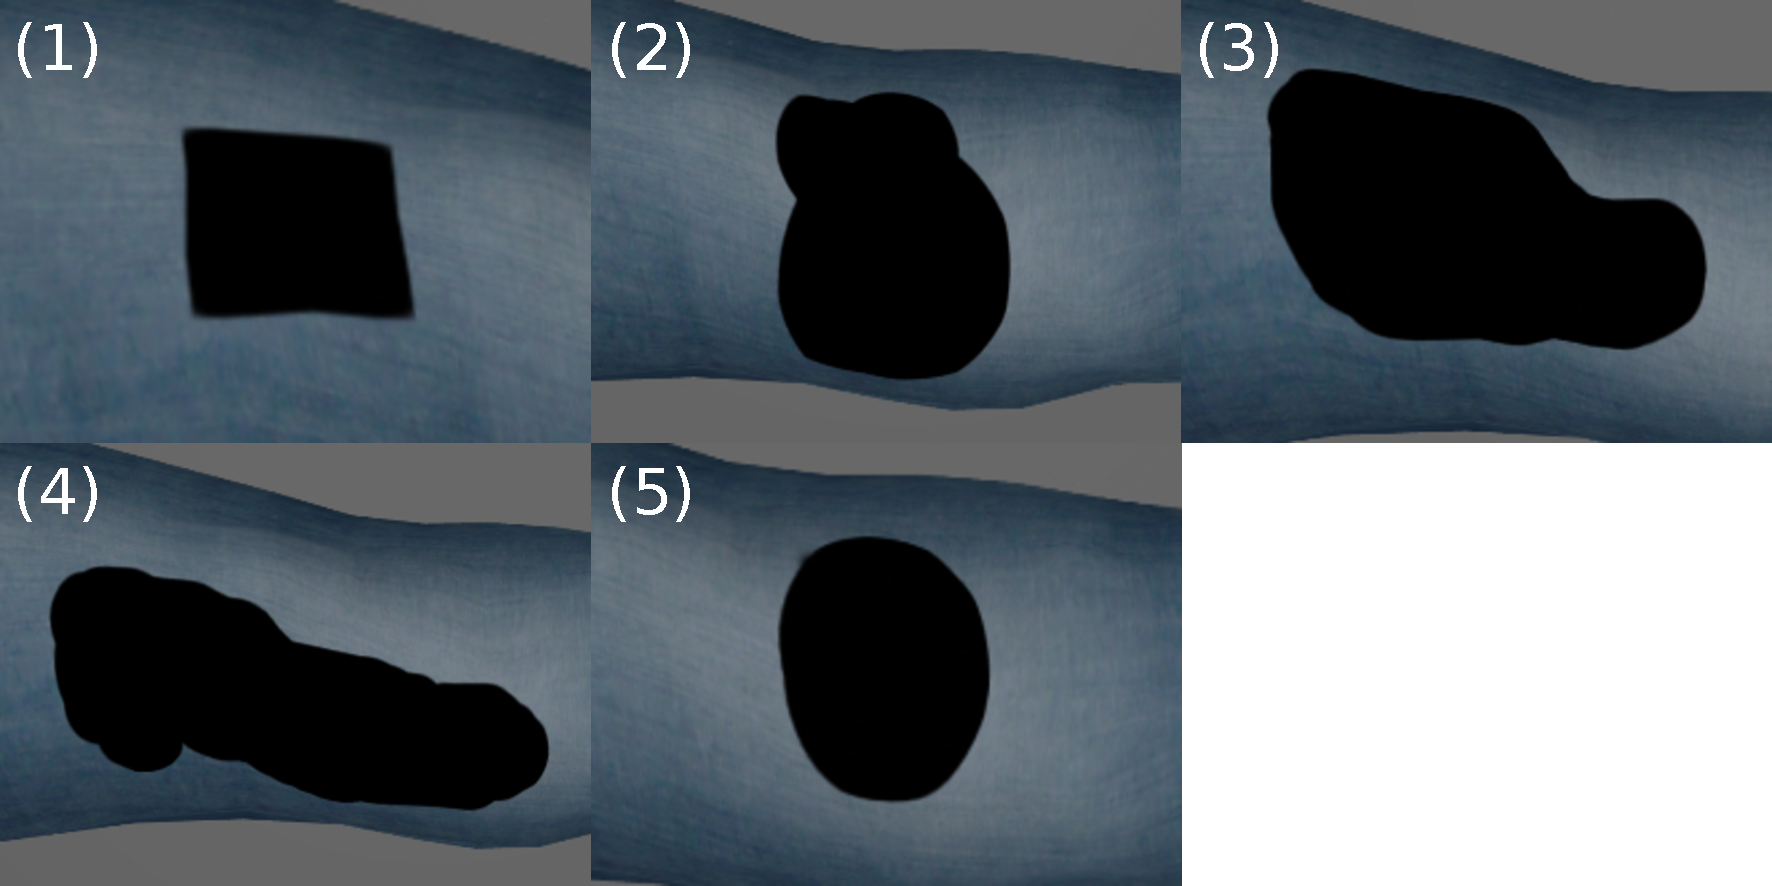
\includegraphics[width=\textwidth]{system_validation_tests_setup_wound_detection_segmentation_wound_models}
	\caption{Wound models used to test wound detection and segmentation. Wounds 1 to 5 were used in simulation. Wound 6 was used on real test environment.}
	\label{fig:system_validation_tests_setup_wound_detection_segmentation_wound_models}
\end{figure}

\begin{figure}[htbp]
	\centering
	\includegraphics[width=\textwidth]{system_validation_tests_setup_wound_detection_segmentation_body_models}
	\caption{Human body models used to represent a patient. (a) Full adult human 3D model. (b) Full adult body mannequin.}
	\label{fig:system_validation_tests_setup_wound_detection_segmentation_body_models}
\end{figure}

% subsection system_validation_tests_setup_wound_detection_segmentation

\subsection{Camera Spatial Data Processing}
\label{subsec:system_validation_tests_setup_camera_spatial_data_processing}

After the wound is detected and segmented, information about its position is needed to control the positioning system. Other geometrical information may be important like area and perimeter. Because non-planar surfaces are considered a mesh of the wound model may provide additional information.

While the area, perimeter and mesh are not essential for the system to work, they add value and may help with autonomy at the higher levels. The position data is essential.

Since there are four types of data obtained, each has its own test.

\subsubsection*{Wound Position}
\label{subsubsec:system_validation_tests_setup_camera_spatial_data_processing_position}

\hspace{.6cm}\textbf{Test description}\\
This test uses a square wound model with a predefined position is space and dimensions. After detection and segmentation of this wound, the position is calculated using the algorithm described in \textbf{Spatial Data Processing} layer on subsection \ref{subsubsec:system_architectural_camera_layers_spatial_data}. The data obtained is compared with the predefined values.\\

\textbf{Pass-fail criteria}\\
The test passes if the following criteria is verified:
\begin{itemize}
    \item the calculated wound poses position match the predefined values within $\pm$ 1 \si{\milli\meter}.
\end{itemize}

The wound model on this test is placed on the robot base plane, both in simulation and real tests. It is a square of $10\times10$ \si{\centi\meter} located at position (0.4, 0, 0) \si{\meter}, referenced to robot base frame.

\subsubsection*{Wound Area}
\label{subsubsec:system_validation_tests_setup_camera_spatial_data_processing_area}

\hspace{.6cm}\textbf{Test description}\\
For this test everything was the same as the position test, except the calculation, which was the area in this case.\\

\textbf{Pass-fail criteria}\\
The test passes if the following criteria is verified:
\begin{itemize}
    \item the calculated area matches the predefined value within $\pm$ 0.1 \si{\meter\squared}.
\end{itemize}
 
% subsubsection system_validation_tests_setup_camera_spatial_data_processing_area

\subsubsection*{Wound Perimeter}
\label{subsubsec:system_validation_tests_setup_camera_spatial_data_processing_perimeter}

\hspace{.6cm}\textbf{Test description}\\
The wound perimeter test is similar to wound position and area tests. The only change is the calculation of the wound perimeter in this case.\\

\textbf{Pass-fail criteria}\\
The test passes if the following criteria is verified:
\begin{itemize}
    \item the calculated perimeter matches the predefined value within $\pm$ 0.01 \si{\meter}.
\end{itemize}
 
% subsubsection system_validation_tests_setup_camera_spatial_data_processing_perimeter

\subsubsection*{Wound Mesh}
\label{subsubsec:system_validation_tests_setup_camera_spatial_data_processing_mesh}

\hspace{.6cm}\textbf{Test description}\\
To test wound mesh generation, the wound models used were the same as the ones used for wound detection and segmentation tests. Since a mesh is useful to explore non-planar surfaces, it makes sense to use non-planar wound models.

The test uses the point data from wound segmentation and applies an algorithm to generate a wound mesh. The validation is done through visual comparison of the mesh shape and wound model shape.\\

\textbf{Pass-fail criteria}\\
The test passes if the following criteria is verified:
\begin{itemize}
    \item the mesh shape empirically matches the wound shape. 
\end{itemize}
 
% subsubsection system_validation_tests_setup_camera_spatial_data_processing_mesh

% subsection system_validation_tests_setup_camera_spatial_data_processing

\subsection{Robot Spatial Data Processing}
\label{subsec:system_validation_tests_setup_robot_spatial_data_processing}

When using the system in co-manipulation the wound detection and segmentation is done by the operator. The robotic arm is manipulated to mark points on the wound contour. After the wound contour is defined, all the data obtained is the same as with the camera. Having this into consideration the wound position test is not done because the position is obtained directly through robotic arm manipulation. The other tests are the same as with the camera. Refer to subsection \ref{subsec:system_validation_tests_setup_camera_spatial_data_processing}.\\
-
The wound model for the other tests is placed on the robot base plane. It is a square of $10\times10$ \si{\centi\meter} located at position (0.4, 0, 0) \si{\meter}, referenced to robot base frame.

These tests are only done on the real environment because of the robotic arm manipulation.

% subsection system_validation_tests_setup_robot_spatial_data_processing

\subsection{Path Planning}
\label{subsec:system_validation_tests_setup_path_planning}

The path planning is essential to define a robot movement capable of direct wound filling 3D bioprinting. The 3 different paths provided must be validated for proper execution.\\

\textbf{Test description}\\
The wound models are the same as the ones for wound detection and segmentation tests. For each wound model, the three path planning algorithms are applied.\\

\textbf{Pass-fail criteria}\\
The test passes if the following criteria are verified:
\begin{itemize}
    \item the planned path is contained inside the wound area;
    \item the planned path can completely cover the whole segmented area.
\end{itemize}

% subsection system_validation_tests_setup_path_planning

\subsection{Trajectory Generation}
\label{subsec:system_validation_tests_setup_trajectory_generation}

A trajectory is the conversion of a path into a movement profile that takes into consideration time, and with speed and acceleration. The generated trajectories need to be tested to verify if they respect speed and acceleration limits, and execution time.\\

\textbf{Test description}\\
The wound models are the same as the ones for wound detection and segmentation tests. For each wound model, the three path planning algorithms are applied. From each path, various trajectories will be generated with both methods (polynomial and \gls{lspb}) and different execution times. \\

\textbf{Pass-fail criteria}\\
The test passes if the following criteria are verified:
\begin{itemize}
    \item the execution time is respected;
    \item the total number of poses respects equation \ref{eq:n_intermediate_trajectory_points};
    \item speed and acceleration limits are respected.
\end{itemize}

These tests are done on simulation and real environments.

% subsection system_validation_tests_setup_trajectory_generation

\subsection{Bioink Management}
\label{subsec:system_validation_tests_setup_bioink_management}

Bioink management is the control of the available bioink volume. It is done via two end-course buttons and the control of syringe plunger movement step. It is important to test the functionality to garantee that the system is able to access its available bioink and act accordingly, for example, stopping the print when it is empty.\\

\textbf{Test description}\\
The tests are done first with the print head only and then with the whole system during a print. With the print head only, the tests moves the empty syringe plunger all the way to the end and waits for motor movement to stop.
The whole system test uses a long path where the bioink would reach the end before the path ends. When it does, both the print head motor and robot movement should stop.\\

\textbf{Pass-fail criteria}\\
The test passes if the following criteria are verified:
\begin{itemize}
    \item the print head motor stops when the plunger reaches all the way in;
    \item the system receives a end-course notification;
    \item the robot trajectory stops when system is notified.
\end{itemize}

These tests are done on the real environment only. The bioprinting system is only implemented and tested with real hardware.

% subsection system_validation_tests_setup_bioink_management

\subsection{Bioink Dispensing}
\label{subsec:system_validation_tests_setup_bioink_dispensing}

Bioink dispensing is the printing action itself. Whenever the system is actively printing it must dispense bioink. After receiving a START command the dispensing should happen until a STOP command is received or an empty bioink condition occurs. Testing this is important to guarantee that the dispensing only happens at the right moment, saving bioink.\\

\textbf{Test description}\\
The tests consist in following two paths, one that is short and the bioink does not reach the end. The other is long and the bioink container will be empty. The dispensing state is evaluated at the end of the first path and at the moment it becomes empty on the second.\\

\textbf{Pass-fail criteria}\\
The test passes if the following criteria are verified:
\begin{itemize}
    \item the dispensing stops at the end of first path (short);
    \item the dispensing stops when the bioink reaches the end.
\end{itemize}

These tests are done on the real environment only. The bioprinting system is only implemented and tested with real hardware.

% subsection system_validation_tests_setup_bioink_dispensing

\subsection{3D Bioprinting Directly on Wound}
\label{subsec:system_validation_tests_setup_bioprinting_directly_wound}

The final test comprises a combination of all the previous functionalities to reach the end goal of bioprinting directly on a wound. The whole procedure will be measured by the final result, i.e., the bioprint itself.\\

\textbf{Test description}\\
For these tests, the six wound models, five for simulation and one for real, will be used. The test has the following steps:

\begin{enumerate}
    \item Position wound into camera FOV;
    \item Run wound detection \& segmentation;
    \item Process wound spatial data;
    \item Generate wound filling path and trajectory;
    \item Execute trajectory;
    \item Dispense bioink during wound filling trajectory section.
\end{enumerate}

\textbf{Pass-fail criteria}\\
The test passes if the following criteria are verified:
\begin{itemize}
    \item the print covers the whole wound area;
    \item the gaps between lines should not be greater than 1 \si{\milli\meter};
    \item the robotic arm position tracking error is less than 1 \si{\milli\meter} {\color{red} ver melhor}.
    \item {\color{red} ver se não há mais critérios}.
\end{itemize}

% subsection system_validation_tests_setup_bioprinting_directly_wound

% section system_validation_tests_setup

% ==========================
% = Simulation Results =
% ==========================

\section{Simulated System Results}
\label{sec:system_validation_simulation_results}

On this section, the results for simulated environment tests are presented. The tests were conducted on Gazebo robot simulator. Gazebo uses a physical simulation engine, advanced 3D graphics, and supports various sensors and robot models. For more information about Gazebo and system setup on Gazebo refer to appendix \ref{app:gazebo_setup}.

The environment consists on a virtual patient room. In it, a patient is lying on bed and the robotic arm lies by the bed side. The room setup tries to replicate a normal patient room with some common hospital apparel (Fig. \ref{fig:system_validation_simulation_gazebo_environment}).

\begin{figure}[htbp]
	\centering
	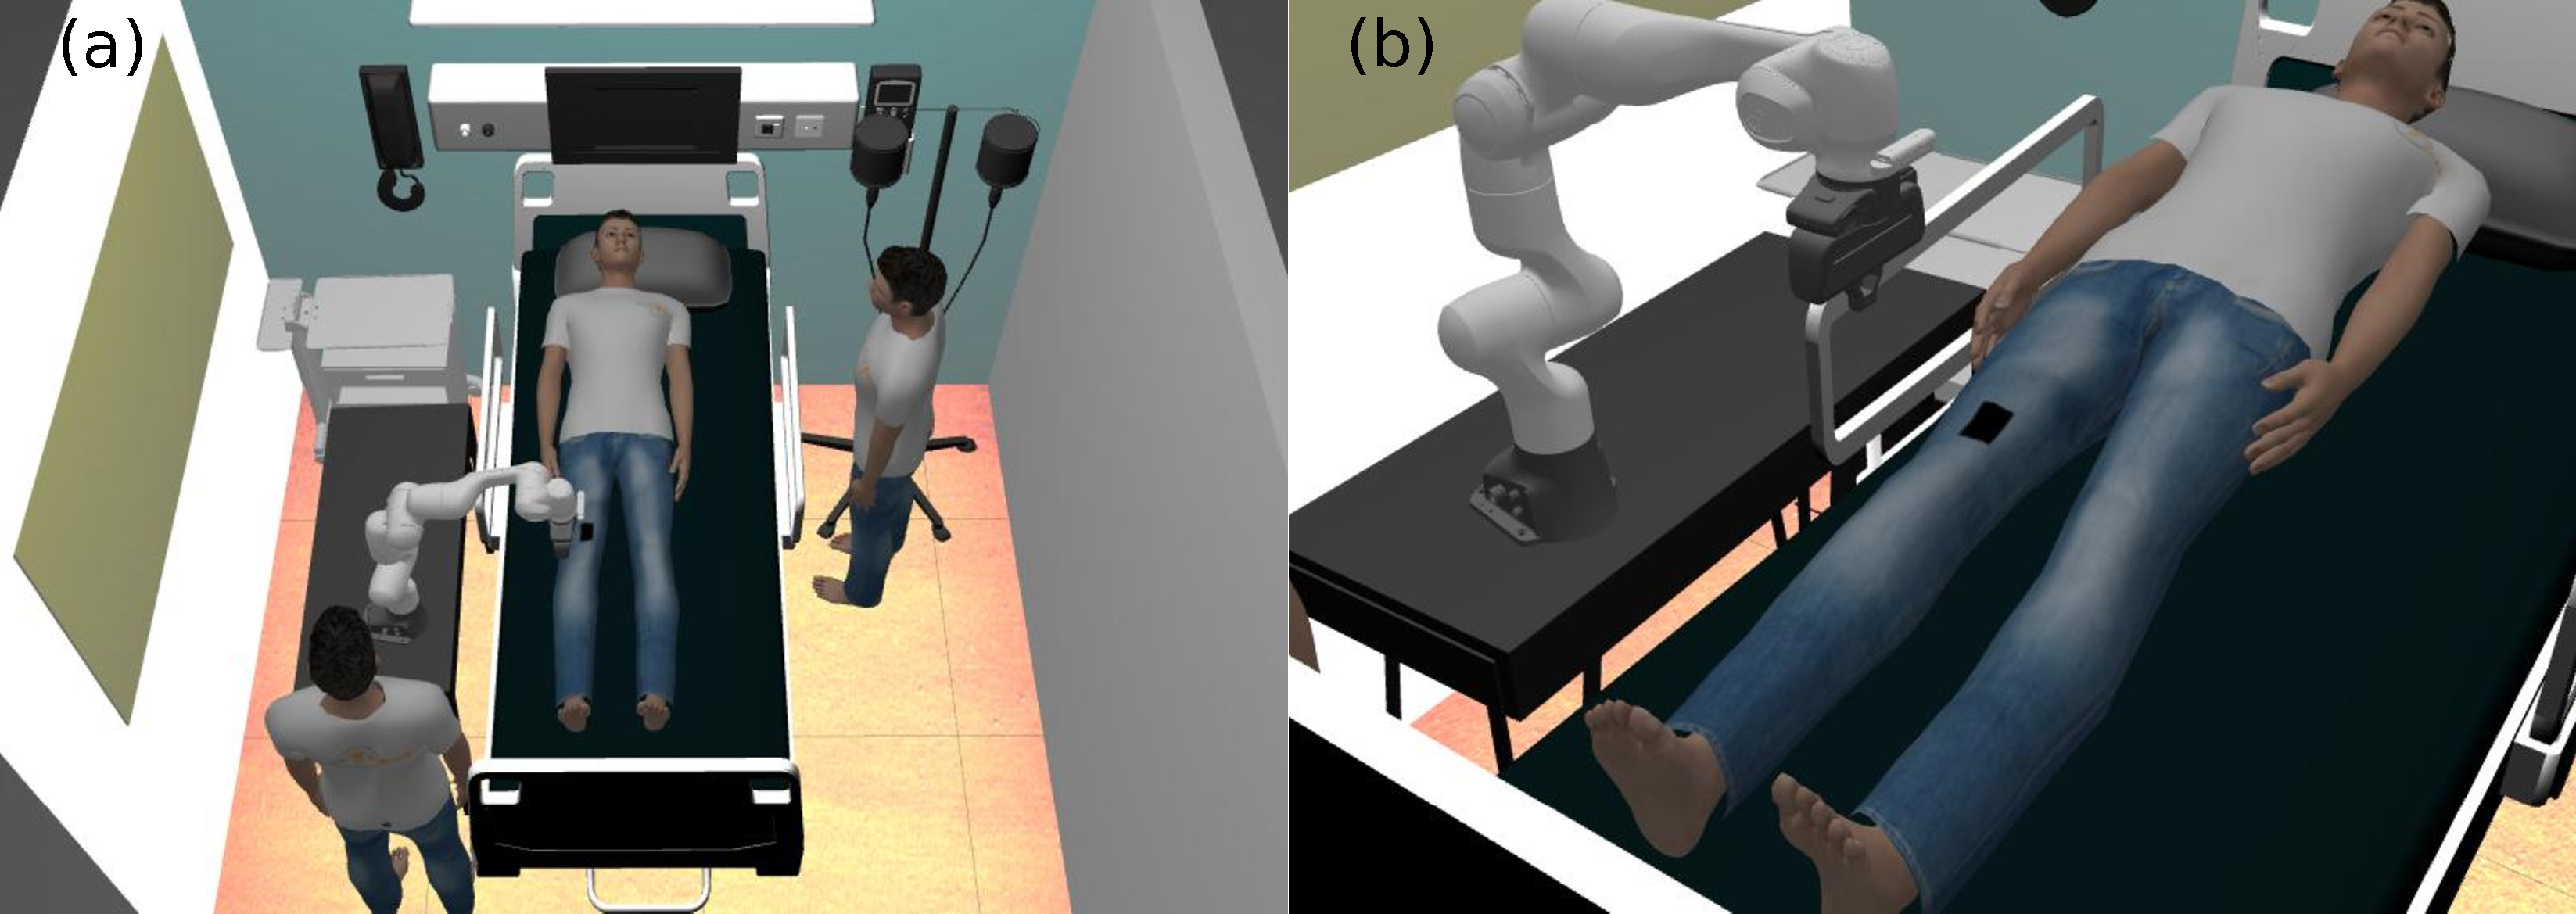
\includegraphics[width=\textwidth]{system_validation_simulation_gazebo_environment}
	\caption{Simulated environment on Gazebo Simulator. (a) Top-view of the patient room. Gives an overall view of the room's apparel organisation. The standing human models represent clinicians. (b) Close-up on robot and patient. The wound model is better visible and its spacial relation with the patient and robot.}
	\label{fig:system_validation_simulation_gazebo_environment}
\end{figure}

\subsection{Wound Detection \& Segmentation}
\label{subsec:simulated_system_results_wound_detection_segmentation}

After running the camera detection and segmentation algorithm on the five wound models supplied, the following results were obtained (Fig. \ref{fig:system_validation_simulation_results_wound_detection_segmentation}).\\

\begin{figure}[htbp]
	\centering
	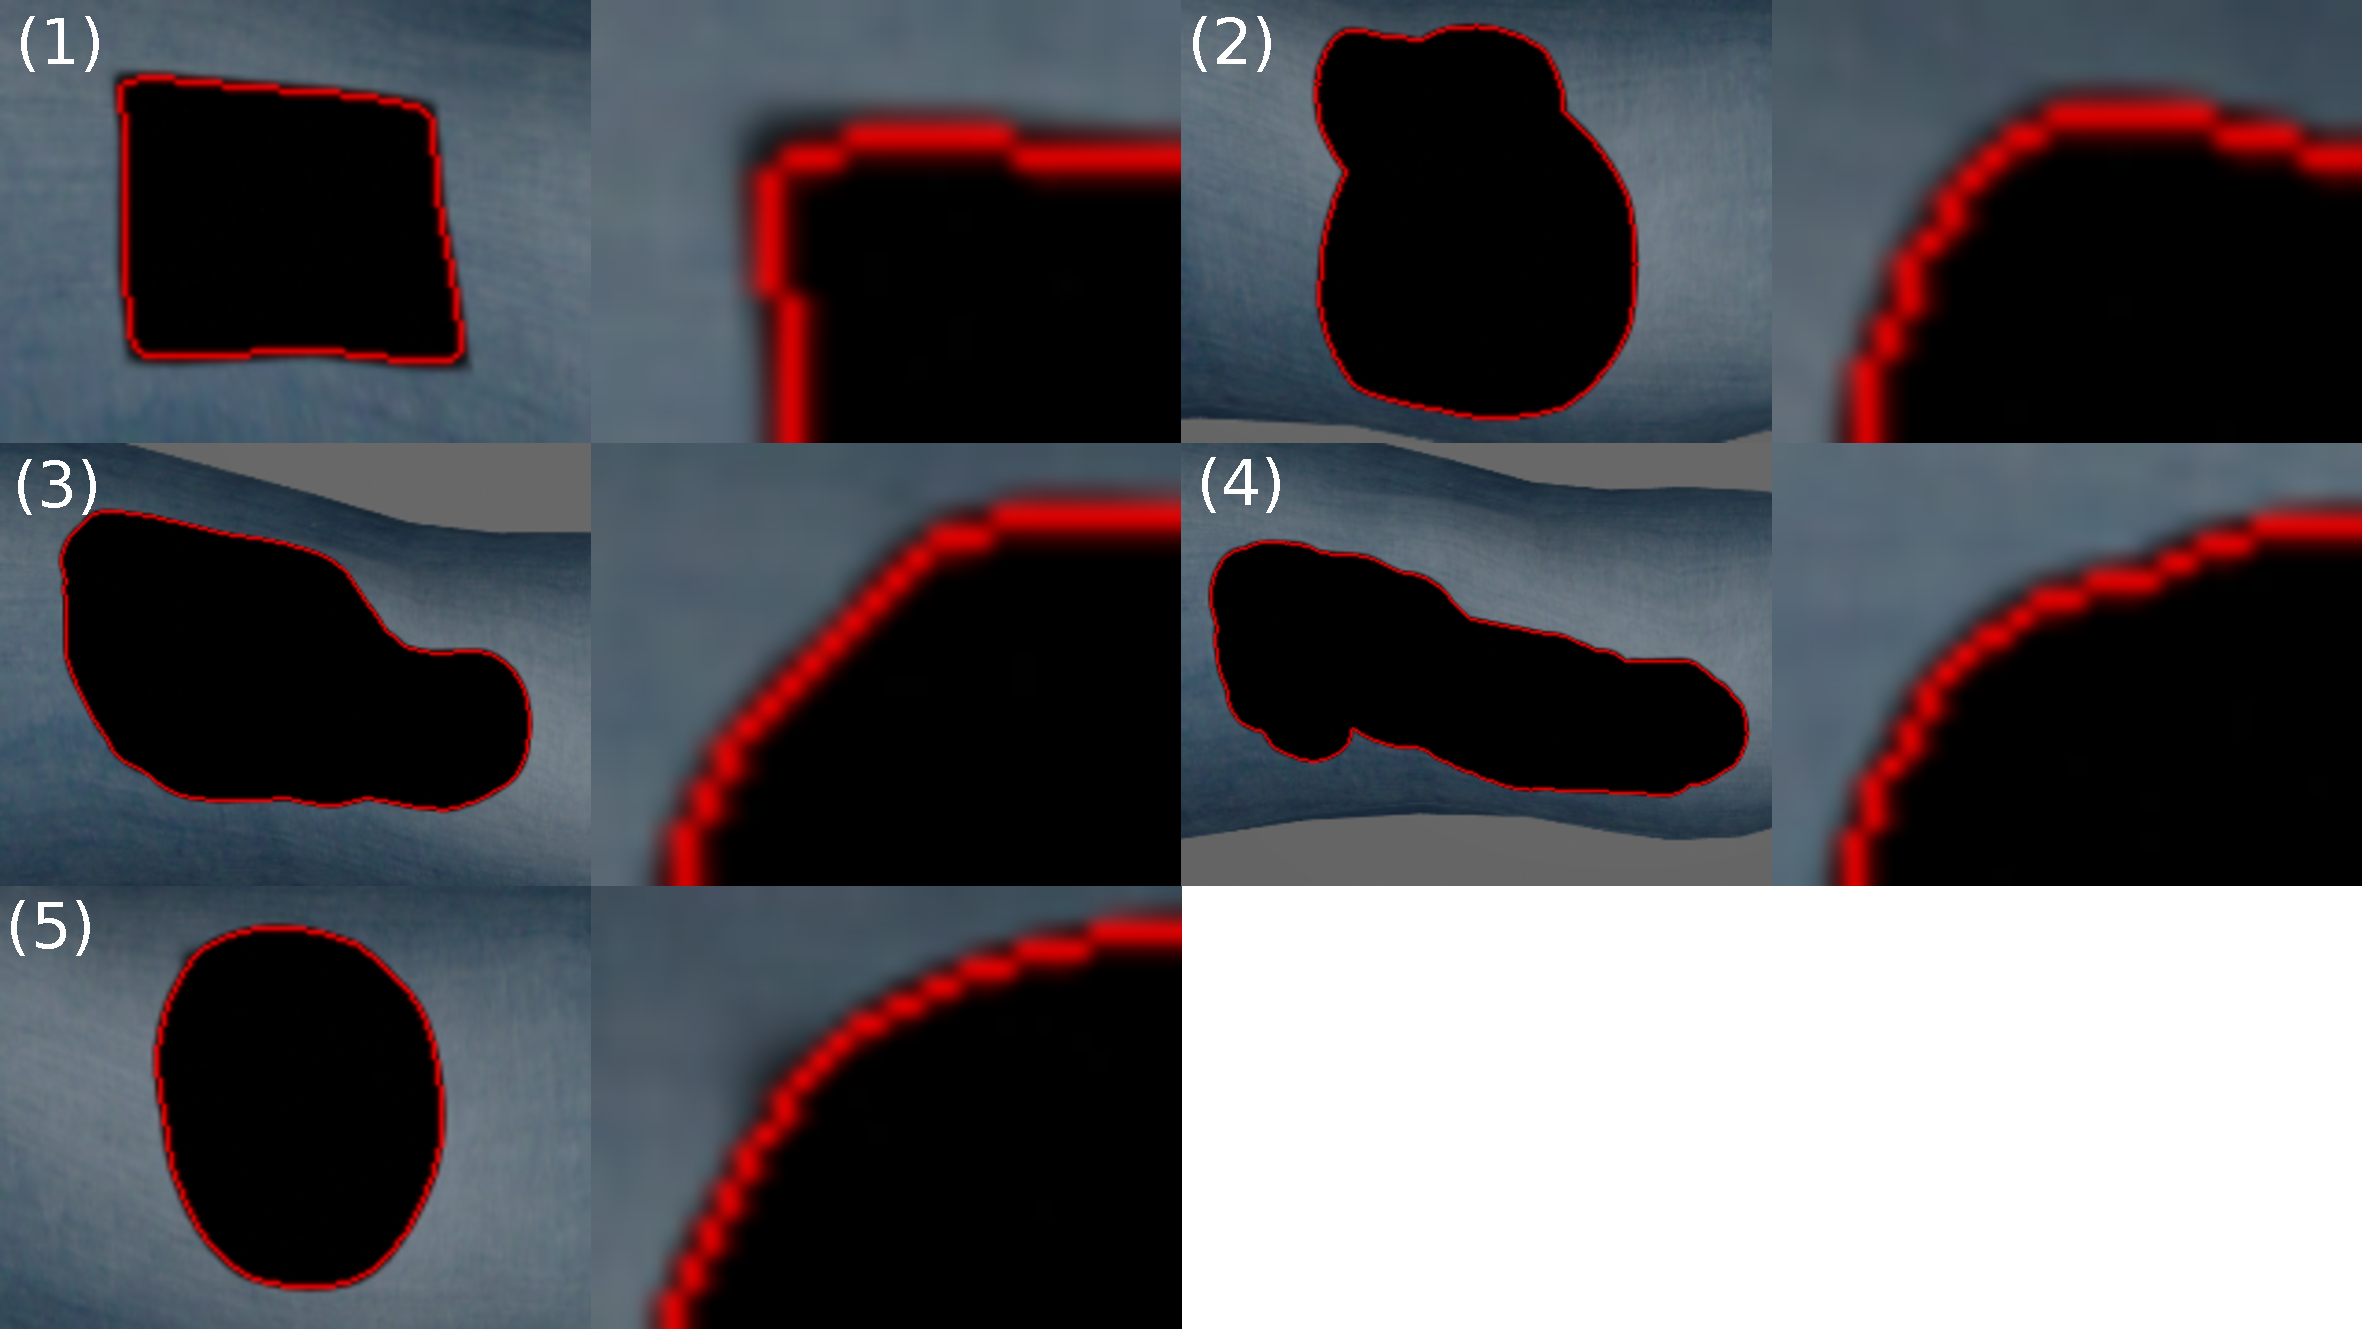
\includegraphics[width=\textwidth]{system_validation_simulation_results_wound_detection_segmentation}
	\caption{Simulated system wound detection \& segmentation results. The red lines are the detected wound contours. Each model has a full image (left) and a detailed crop (right) to see the wound-contour edge relation. It is visible that for every wound model the contour encloses the whole wound.}
	\label{fig:system_validation_simulation_results_wound_detection_segmentation}
\end{figure}

On all models, the algorithm was able to correctly detect the wound model and segment it. The segmentation contour encloses the whole wound area as desired. The detailed crops for each wound show that the contour goes all the way to the edge of the wound model. The algorithm verified the test criteria.

% subsection simulated_system_results_wound_detection_segmentation

\subsection{Camera Spatial Data Processing}
\label{subsec:simulated_system_results_camera_spatial_data_processing}

After the wound is detected and segmented and a contour is created, spatial data can be obtained. Camera spatial data processing encompasses various tests. The results will be presented for each test separately.

\subsubsection*{Wound Position}
\label{subsubsec:simulated_system_results_camera_spatial_data_processing_position}

% subsubsection simulated_system_results_camera_spatial_data_processing_position

\subsubsection*{Wound Area}
\label{subsubsec:simulated_system_results_camera_spatial_data_processing_area}

% subsubsection simulated_system_results_camera_spatial_data_processing_area

\subsubsection*{Wound Perimeter}
\label{subsubsec:simulated_system_results_camera_spatial_data_processing_perimeter}

% subsubsection simulated_system_results_camera_spatial_data_processing_perimeter

\subsubsection*{Wound Mesh}
\label{subsubsec:simulated_system_results_camera_spatial_data_processing_mesh}

For the wound mesh tests, each wound model will have a point cloud and a mesh associated. The mesh is obtained from the point cloud. The point clouds are visualized on RViz (for more information refer to annex \ref{ann:ros}) and the meshes on MeshLab. The results are presented on Figure \ref{fig:simulation_test_results_camera_spatial_data_wound_pcloud_mesh_resume}.

\begin{figure}[htbp]
	\centering
	\includegraphics[width=\textwidth]{simulation_test_results_camera_spatial_data_wound_pcloud_mesh_resume}
	\caption{}
	\label{fig:simulation_test_results_camera_spatial_data_wound_pcloud_mesh_resume}
\end{figure}

% subsubsection simulated_system_results_camera_spatial_data_processing_mesh

% subsection simulated_system_results_camera_spatial_data_processing

\subsection{Path Planning}
\label{subsec:simulated_system_results_path_planning}

With the wound contour available, the path planning algorithms can be applied. Three different algorithms with configuration were applied to each wound model. The results are presented on Figure \ref{fig:simulation_test_results_toolpath_resume}.\\

\begin{figure}[htbp]
	\centering
	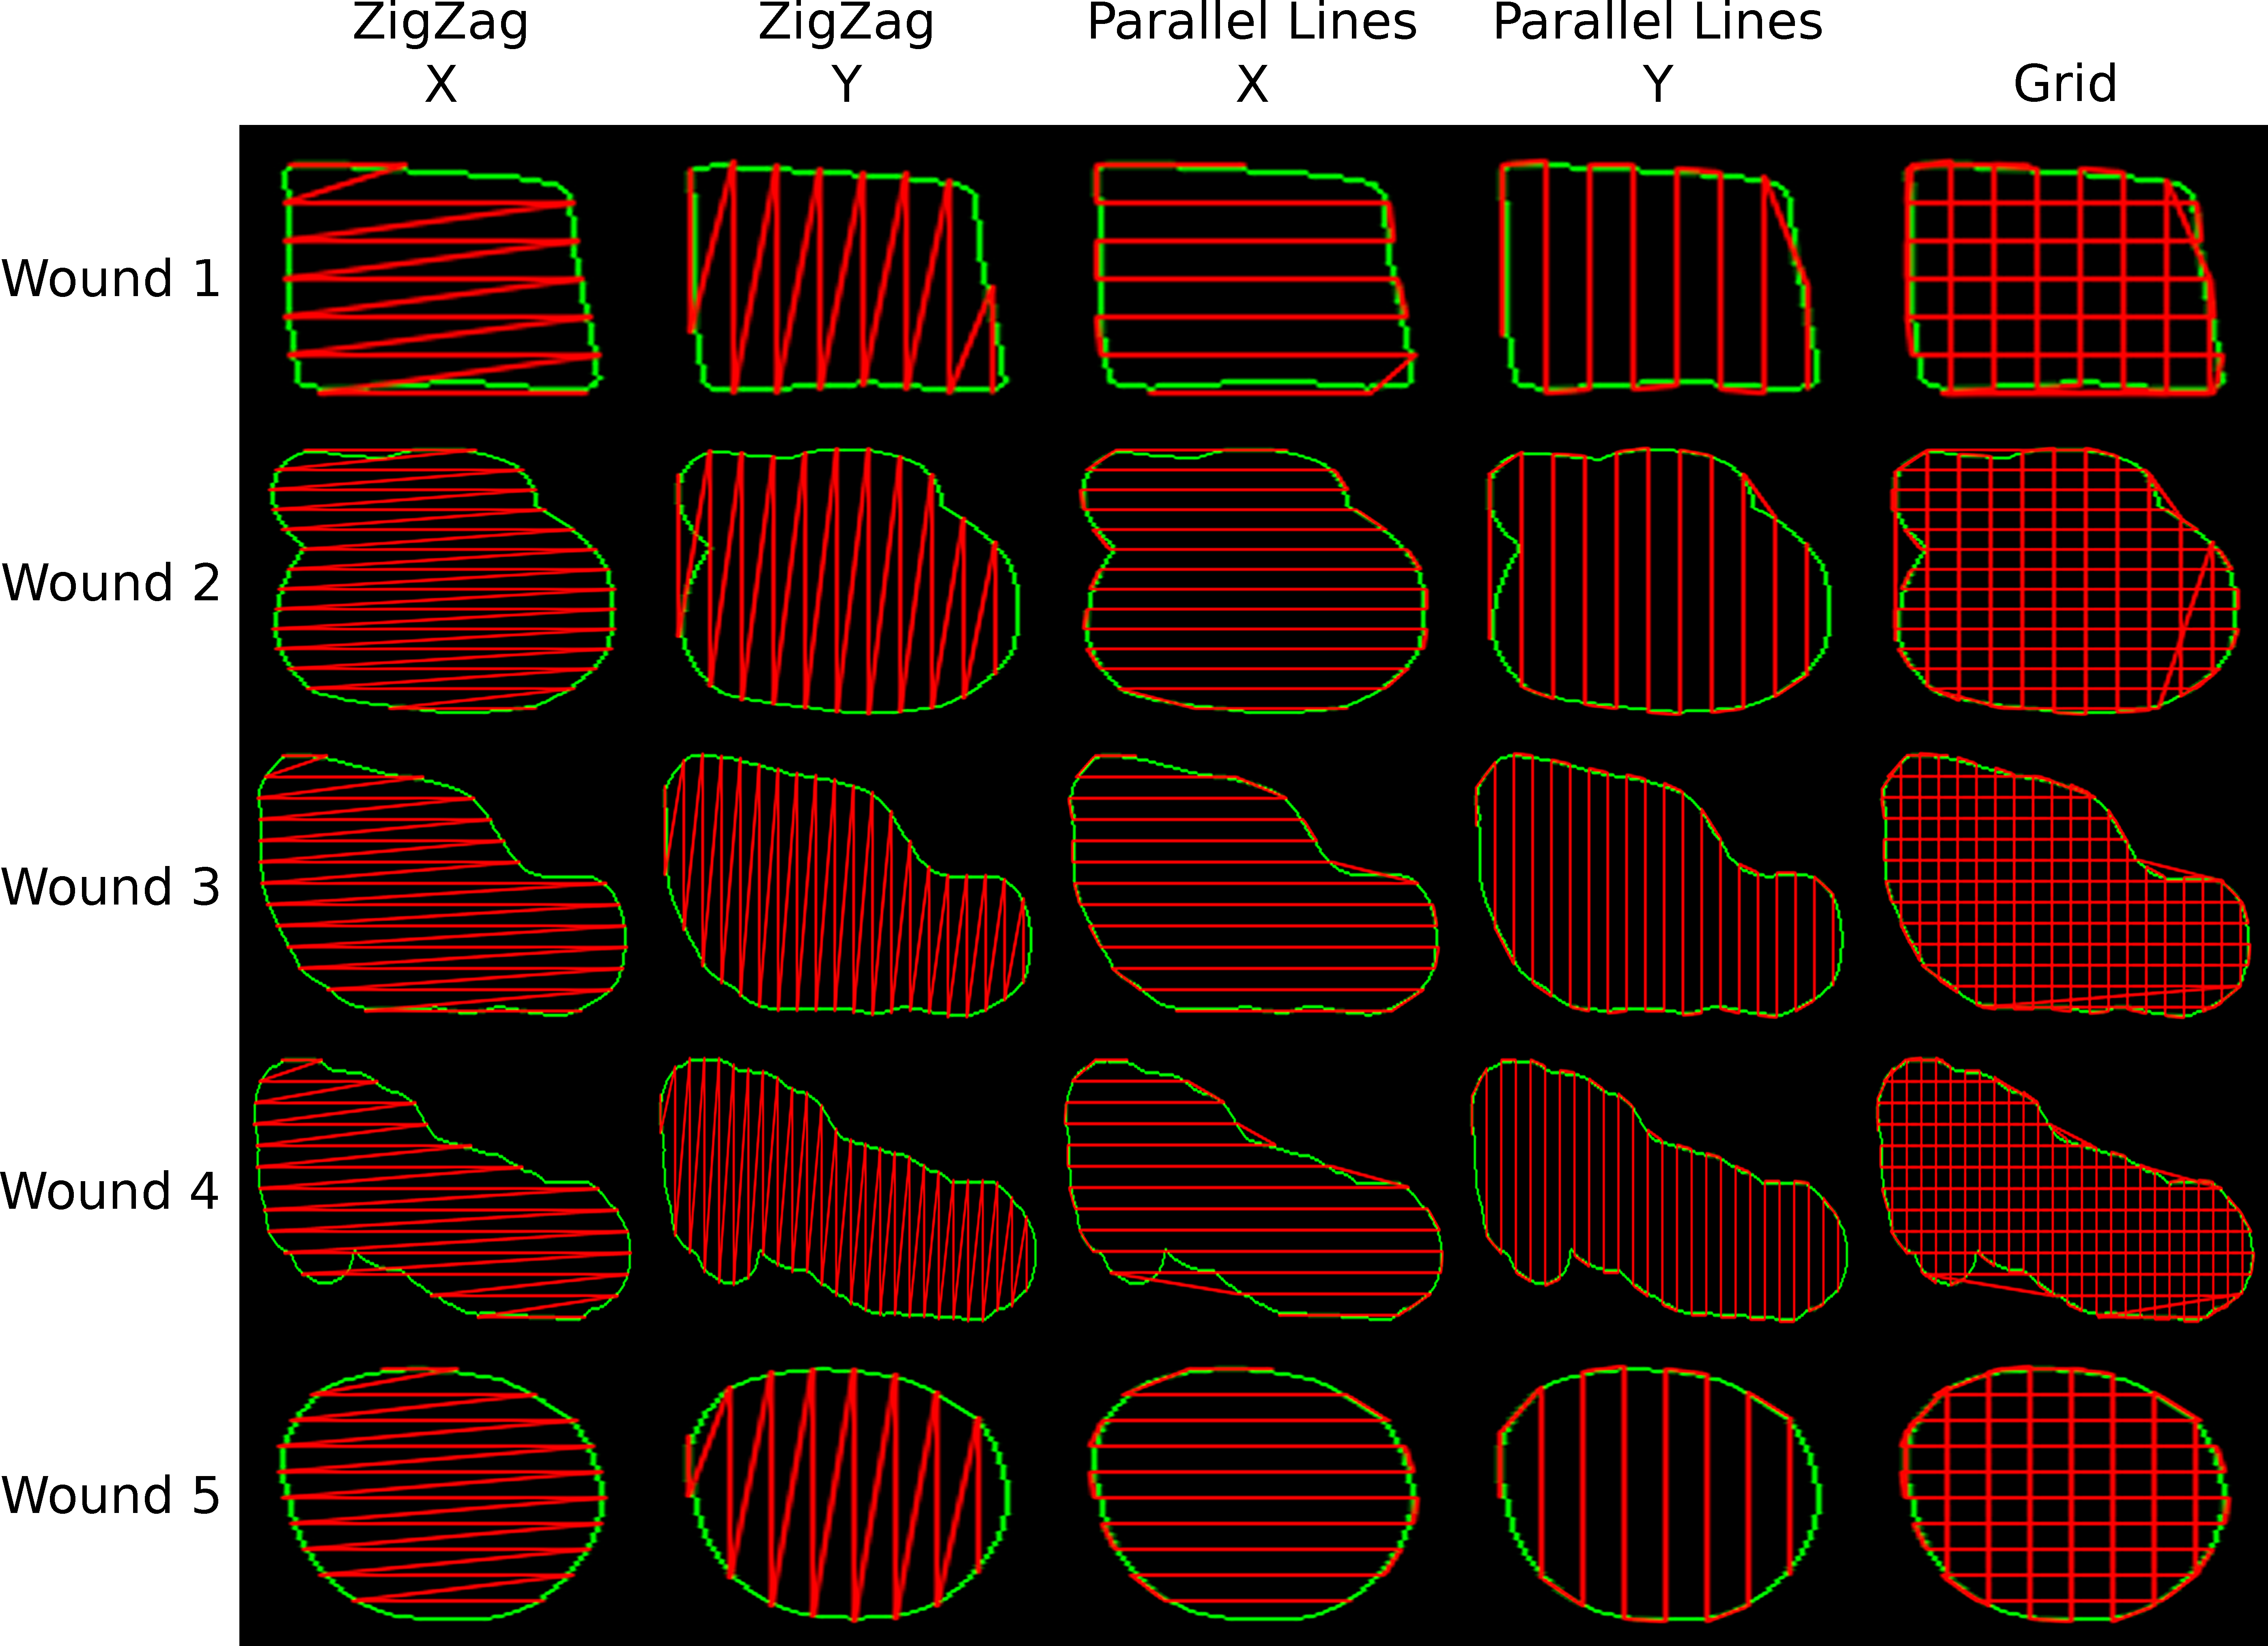
\includegraphics[width=\textwidth]{simulation_test_results_toolpath_resume}
	\caption{Simulation results for path planning. Each line represents a different wound model. From left to right, the algorithm changes. All results have a distance between lines, $L = 5$, in pixels.}
	\label{fig:simulation_test_results_toolpath_resume}
\end{figure}

All the results show that the planned paths are contained inside the wound area. They are also able of filling the wound completely. By controlling the distance $L$, various filling grades can be accomplished. The examples presented show a fixed value of $L = 5$. The test criteria are satisfied.

However, it is important to mention that in some cases the planned path goes beyond the wound segmented area. This happens in zones where the shape is concave, but it also depends on the orientation of the algorithm and distance $L$. For example, wound 4's ZigZag X path goes outside the segmented area, while the ZigZag Y does not.\\

The full results with various path configurations are available on appendix \ref{app:simulation_test_results}.

% subsection simulated_system_results_path_planning

\subsection{Trajectory Generation}
\label{subsec:simulated_system_results_trajectory_generation}

% subsection simulated_system_results_trajectory_generation

\subsection{3D Bioprinting Directly on Wound}
\label{subsec:simulated_system_results_bioprinting_directly_wound}

% subsection simulated_system_results_bioprinting_directly_wound

% section system_validation_simulation_results

% ==========================
% = Real Results =
% ==========================

\section{Real System Results}
\label{sec:system_validation_real_results}

On this section, the results for the real environment tests are presented.

\subsection{Wound Detection \& Segmentation}
\label{subsec:real_system_results_wound_detection_segmentation}

After running the camera detection and segmentation algorithm on the wound model supplied, the following results were obtained (Fig. \ref{fig:system_validation_real_results_wound_detection_segmentation}).\\

\begin{figure}[htbp]
	\centering
	\includegraphics[width=\textwidth]{system_validation_real_results_wound_detection_segmentation}
	\caption{Real system wound detection \& segmentation results.}
	\label{fig:system_validation_real_results_wound_detection_segmentation}
\end{figure}

% subsection real_system_results_wound_detection_segmentation

\subsection{Camera Spatial Data Processing}
\label{subsec:real_system_results_camera_spatial_data_processing}

% subsection real_system_results_camera_spatial_data_processing

\subsection{Path Planning}
\label{subsec:real_system_results_path_planning}

% subsection real_system_results_path_planning

\subsection{Trajectory Generation}
\label{subsec:real_system_results_trajectory_generation}

% subsection real_system_results_trajectory_generation

\subsection{Bioink Management}
\label{subsec:real_system_results_bioink_management}

% subsection real_system_results_bioink_management

\subsection{Bioink Dispensing}
\label{subsec:real_system_results_bioink_dispensing}

% subsection real_system_results_bioink_dispensing

\subsection{3D Bioprinting Directly on Wound}
\label{subsec:real_system_results_bioprinting_directly_wound}

% subsection real_system_results_bioprinting_directly_wound

% section system_validation_real_results

% ==========================
% = Discussion =
% ==========================

\section{Discussion}
\label{sec:system_validation_discussion}

{\color{red} All the data obtained for the wounds with the camera depend completely on the camera orientation. If the camera detects the wound but is not at the best angle, the detection may be partial which means the whole wound filling procedure will fail.}

{\color{red} The area & perimeter calculation may work well on planar wounds but it will fail on non-planar wounds. It depends heavily on the camera orientation. The mesh is probably the best tool to measure the area and perimeter correctly.}

% section system_validation_discussion